% =====================================================================
%  TEMPLATE PROPOSAL SKRIPSI
%  S1 Rekayasa Sistem Komputer, Fakultas Teknik, UM Buton
%  Kompilasi PDF : xelatex (lihat menu.sh)   |   Word : pandoc (lihat menu.sh)
%  Ukuran dan tata letak sama dengan Seminar Hasil dan Skripsi: A4; margin kiri/atas/kanan/bawah
%  = 4/4/3/3 cm; Times New Roman 12 pt; 1,5 spasi; judul "BAB I" di tengah, tiap bab mulai halaman baru.
%  Isi dipisah per bab di folder bab/ ; ubah isi di sana.
% =====================================================================
\documentclass[12pt,a4paper]{report}
\usepackage{skripsi}
\usepackage{skripsi-bab}

% ---------- Data dosen & peran (common/dosen.tex, common/peran.tex) ----------
% =====================================================================
%  DAFTAR DOSEN  --  Program Studi Rekayasa Sistem Komputer, UM Buton
%  Satu dosen = dua makro:  \dsnKunci (nama dan gelar)  dan  \nidnKunci (NIDN).
%  Tambah dosen baru dengan menyalin dua baris di bawah. Peran (pembimbing, penguji, dst.)
%  diatur di peran.tex atau lewat  ./menu.sh  ->  "Atur dosen / peran".
% =====================================================================
\newcommand{\dsnAwaluddin}{Muhammad Awaluddin, S.Kom., M.Kom}
\newcommand{\nidnAwaluddin}{0909038201}
\newcommand{\dsnDarmawan}{Darmawan, S.Kom., M.Kom}
\newcommand{\nidnDarmawan}{0911048204}
\newcommand{\dsnRando}{Rando, S.Kom., M.Eng.}
\newcommand{\nidnRando}{0911069501}
\newcommand{\dsnSaidi}{La Ode Muhammad Saidi, S.Si., M.Kom}
\newcommand{\nidnSaidi}{0913038905}
\newcommand{\dsnDidin}{Didin Adri, S.Si., M.Sc}
\newcommand{\nidnDidin}{0930088802}
\newcommand{\dsnHibrian}{Muhammad Hibrian Wiwi, S.T., M.Kom}
\newcommand{\nidnHibrian}{0930129003}
\newcommand{\dsnRasyid}{Muhammad Abdur Rasyid Asruddin, S.T., M.Kom}
\newcommand{\nidnRasyid}{6641774675130242}
% Dekan Fakultas Teknik
\newcommand{\dsnAgusman}{Agusman, S.T., M.M}
\newcommand{\nidnAgusman}{0917088206}

% =====================================================================
%  PERAN DOSEN  --  dipakai otomatis di sampul, lembar persetujuan/pengesahan,
%  kata pengantar, dan abstrak semua dokumen.
%  Isi dengan kunci dosen dari dosen.tex, mis.  \dsnAwaluddin  dan  \nidnAwaluddin.
%  Atau jalankan  ./menu.sh  lalu pilih "Atur dosen / peran"  (berkas ini ditulis ulang otomatis).
% =====================================================================
\newcommand{\PembimbingI}{…………………}\newcommand{\PembimbingInidn}{……………………}
\newcommand{\PembimbingII}{…………………}\newcommand{\PembimbingIInidn}{……………………}
\newcommand{\PengujiI}{…………………}\newcommand{\PengujiInidn}{……………………}
\newcommand{\PengujiII}{…………………}\newcommand{\PengujiIInidn}{……………………}
\newcommand{\KetuaProdi}{…………………}\newcommand{\KetuaProdinidn}{……………………}
\newcommand{\Dekan}{\dsnAgusman}\newcommand{\Dekannidn}{\nidnAgusman}


% ---------- Makro yang ikut dibaca pandoc ----------
\newcommand{\logo}[1]{
\includegraphics[width=#1]{../gambar/logo-umbuton.png}}
\newcommand{\babtp}[1]{\chapter*{#1}\addcontentsline{toc}{chapter}{#1}}
\definecolor{gantt}{HTML}{FF9900}
\newcommand{\isi}{\cellcolor{gantt}\textbf{~}}   % sel terisi pada jadwal

\begin{document}

% Tambah bab baru: buat berkas bab/NN-nama.tex lalu \input di sini.
% Sampul dan lembar persetujuan pembimbing
% ============================ SAMPUL ============================
\thispagestyle{empty}
\begin{ruang}{0.4}\end{ruang}
\begin{sampulbesar}
\textbf{PROPOSAL SKRIPSI}
\end{sampulbesar}
\begin{ruang}{0.5}\end{ruang}
\begin{sampulbesar}
\textbf{JUDUL PROPOSAL SKRIPSI}
\end{sampulbesar}
\begin{ruang}{0.6}\end{ruang}
\begin{tengah}
\logo{4.5cm}
\end{tengah}
\begin{ruang}{0.6}\end{ruang}
\begin{sampulsedang}
\textbf{Disusun oleh:}

\textbf{Nama Mahasiswa/i}

\textbf{NPM}
\end{sampulsedang}
\begin{ruang}{0.8}\end{ruang}
\begin{sampulsedang}
\textbf{PROGRAM STUDI REKAYASA SISTEM KOMPUTER}

\textbf{FAKULTAS TEKNIK}

\textbf{UNIVERSITAS MUHAMMADIYAH BUTON}

\textbf{BAUBAU}

\textbf{202x}
\end{sampulsedang}
\begin{halamanbaru}\end{halamanbaru}

% ============================ LEMBAR PERSETUJUAN ============================
\thispagestyle{empty}
\begin{tengah}
\textbf{\underline{PROPOSAL SKRIPSI}}
\end{tengah}

\begin{tanpagaris}
\begin{longtable}{@{}p{0.16\linewidth}p{0.04\linewidth}p{0.74\linewidth}@{}}
Nama & : & ………………………………………………………… \\[6pt]
NPM & : & ………………………………………………………… \\[6pt]
\textit{Contact} & : & ………………………………………………………… \\[6pt]
 & & ………………………………………………………… \\
 & & {\footnotesize (alamat, telepon, email untuk kemudahan menghubungi; dan jika ada perubahan data harap segera menghubungi Program Studi)} \\
\end{longtable}
\end{tanpagaris}

\begin{ruang}{1.5}\end{ruang}
\begin{tengah}
\textbf{PERSETUJUAN PEMBIMBING}

Proposal Skripsi ini telah disetujui oleh:
\end{tengah}

\begin{tanpagaris}\begin{tabelpusat}
\begin{longtable}{@{}>{\centering\arraybackslash}p{0.48\linewidth}>{\centering\arraybackslash}p{0.48\linewidth}@{}}
\textbf{Pembimbing I}\newline ~\newline ~\newline ~\newline ~\newline ~\newline ~\newline ~\newline \satubaris{\PembimbingI}\newline NIDN. \PembimbingInidn &
\textbf{Pembimbing II}\newline ~\newline ~\newline ~\newline ~\newline ~\newline ~\newline ~\newline \satubaris{\PembimbingII}\newline NIDN. \PembimbingIInidn \\
\end{longtable}
\end{tabelpusat}\end{tanpagaris}
\begin{akhirsampul}\end{akhirsampul}
      % sampul, lembar persetujuan (tanpa nomor halaman)
% Abstrak (Indonesia dan Inggris): satu paragraf, maksimal 300 kata, satu spasi. Ganti teks dalam [ ... ] dengan isi penelitian Anda.
\babtp{ABSTRAK}
\begin{abstrak}
Penelitian ini dilatarbelakangi oleh [permasalahan utama yang dihadapi dan alasan penelitian perlu dilakukan]. Kondisi tersebut menunjukkan perlunya [solusi atau pendekatan yang diusulkan] agar [tujuan akhir yang ingin dicapai]. Berdasarkan hasil observasi awal dan kajian pustaka, [uraikan kesenjangan antara kondisi yang diharapkan dan kondisi nyata, disertai data atau sitasi pendukung]. Hasil analisis awal menunjukkan bahwa [temuan awal atau studi pendahuluan], sehingga penelitian ini dipandang layak dan mendesak untuk dilaksanakan. Apabila tidak ditangani, [dampak yang mungkin timbul] akan semakin meluas, sehingga diperlukan penelitian yang [karakteristik penelitian yang dibutuhkan]. Permasalahan yang dirumuskan dalam penelitian ini adalah [rumusan masalah pertama], [rumusan masalah kedua], dan [rumusan masalah ketiga]. Tujuan penelitian ini adalah [tujuan penelitian secara ringkas, sesuai rumusan masalah]. Penelitian direncanakan dilaksanakan di [lokasi penelitian] selama [lama penelitian] dengan menggunakan metode [nama metode atau pendekatan]. Tahapan penelitian meliputi [tahap pertama], [tahap kedua], dan [tahap ketiga]. Data akan dikumpulkan melalui [teknik pengumpulan data] dan dianalisis dengan [teknik analisis data]. Sistem atau objek yang diteliti dirancang menggunakan [perangkat keras dan perangkat lunak yang digunakan]. Pengujian akan dilakukan dengan [jumlah] skenario, yaitu [skenario pertama], [skenario kedua], dan [skenario ketiga], masing-masing diulang sebanyak [jumlah pengulangan] kali agar hasilnya dapat diandalkan. Kinerja akan diukur berdasarkan [indikator kinerja], dengan parameter yang diamati meliputi [parameter pertama], [parameter kedua], dan [parameter ketiga] serta nilai acuan [nilai acuan atau standar yang digunakan]. Hasil yang diharapkan dari penelitian ini adalah [hasil utama yang diharapkan beserta target pencapaiannya]. Keterbatasan penelitian ini adalah [batasan penelitian], sehingga hasilnya terutama berlaku pada [cakupan hasil penelitian]. Penelitian ini diharapkan memberikan manfaat bagi [pihak yang memperoleh manfaat] serta menjadi dasar bagi pengembangan penelitian selanjutnya di bidang [bidang ilmu].

\textbf{Kata kunci:} kata kunci 1, kata kunci 2, kata kunci 3.
\end{abstrak}

\begin{halamanbaru}\end{halamanbaru}
\babtp{ABSTRACT}
\begin{abstrak}
This research is motivated by [the main problem and the reason the study is needed]. This condition shows the need for [the proposed solution or approach] in order to [the final goal to be achieved]. Based on preliminary observations and a literature review, [describe the gap between the expected and actual conditions, supported by data or citations]. A preliminary analysis shows that [the initial finding or preliminary study], so this research is considered feasible and urgent. If left unaddressed, [the possible impact] will continue to spread, so research that [the required characteristics of the study] is needed. The problems formulated in this research are [first problem], [second problem], and [third problem]. The objective of this research is [the research objective, consistent with the problem statement]. The research is planned to be carried out at [research location] for [duration] using [method or approach]. The stages of the research include [first stage], [second stage], and [third stage]. Data will be collected through [data collection technique] and analyzed using [data analysis technique]. The system under study is designed using [hardware and software]. Testing will be conducted in [number] scenarios, namely [first scenario], [second scenario], and [third scenario], each repeated [number of repetitions] times to ensure reliable results. Performance will be measured based on [performance indicators], with the observed parameters including [first parameter], [second parameter], and [third parameter] and the reference value of [reference value or standard used]. The expected result of this research is [main expected result and its target]. The limitation of this research is [research limitation], so the results mainly apply to [scope of the results]. This research is expected to benefit [beneficiaries] and to serve as a basis for further research in the field of [field of study].

\textbf{Keywords:} keyword 1, keyword 2, keyword 3.
\end{abstrak}

\begin{halamanbaru}\end{halamanbaru}
     % abstrak (angka romawi)
% Daftar isi, daftar tabel, daftar gambar; setelah ini nomor halaman mulai dari 1 (isi)
\begin{daftarisi}\end{daftarisi}
\begin{daftartabel}\end{daftartabel}
\begin{daftargambar}\end{daftargambar}
\begin{akhirdepan}\end{akhirdepan}
\pagestyle{isi}

  % daftar isi; setelah ini nomor halaman mulai dari 1

% Bab 1  Pendahuluan
\chapter{PENDAHULUAN}

\section{Latar Belakang}
Latar belakang masalah harus menjelaskan rumusan masalah yang akan dibahas dan dicarikan penyelesaiannya. Selain itu, latar belakang masalah juga harus dapat menjelaskan mengapa topik penelitian yang dilakukan dipandang menarik, penting, dan layak untuk diteliti. Berikan data pendukung yang memadai untuk meyakinkan pembaca bahwa penelitian yang Penulis lakukan penting.

Dokumen ini adalah \textit{template} proposal skripsi yang resmi dikeluarkan oleh Rekayasa Sistem Komputer Universitas Muhammadiyah Buton (UM Buton). Dokumen proposal skripsi harus dibuat pada kertas A4 dengan \textit{margin} atas, kanan, bawah, dan kiri secara berurutan adalah 4 cm, 3 cm, 3 cm, dan 4 cm. Format penulisan proposal skripsi adalah \textit{Times New Roman} dengan ukuran \textit{text} 12 pt dan berspasi 1,5 \textit{lines}. Jelaskan penggunaan singkatan dan akronim saat pertama kali muncul. Untuk hitungan yang memiliki angka desimal, gunakan tanda koma (“,”) untuk memisahkan pecahan desimal tersebut, contoh: “0,25; 7,56; …”.

\textit{Contoh kalimat bersitasi:} Penjadwalan paket pada jaringan seluler berperan penting dalam membagi sumber daya radio secara adil di antara pengguna (Capozzi et al., 2013). Andrews (2007) menyatakan bahwa teori penjadwalan pada jaringan data nirkabel terus berkembang seiring bertambahnya kebutuhan layanan. Kebutuhan serupa juga muncul pada jaringan listrik cerdas yang menuntut penjadwalan waktu nyata (Xu \& Fischione, 2012). Data statistik nasional dipublikasikan secara berkala oleh lembaga resmi (Badan Pusat Statistik, 1997).

\section{Rumusan Masalah}
Rumusan masalah diambil berdasarkan uraian latar belakang. Rumusan masalah ditulis dalam bentuk \textit{list}.

\section{Tujuan Penelitian}
Dalam subbab ini disebutkan secara spesifik tujuan penelitian yang ingin dicapai.

\section{Manfaat Penelitian}
Tulis manfaat penelitian yang ingin Penulis capai.

\textit{Contoh kalimat bersitasi:} Perangkat keras yang digunakan mengikuti spesifikasi dari pabrikan (Espressif Systems, 2023).


% Bab 2  Tinjauan Pustaka
\chapter{TINJAUAN PUSTAKA}

\section{Studi Literatur}
Bagian ini memuat ulasan penelitian di bidang sejenis yang telah dilakukan oleh peneliti lain sebelumnya. Anda dapat mencantumkan hal-hal yang telah penulis pelajari dari literatur lain selama melakukan penelitian. Studi literatur sebaiknya menunjukkan pendekatan yang dilakukan oleh peneliti-peneliti sebelumnya dalam menjawab permasalahan penelitian. Semua sumber literatur yang digunakan di dalam subbab ini harus dicantumkan. Sitasi di dalam teks menggunakan gaya APA (\textit{American Psychological Association}) edisi ke-7 dengan format penulis--tahun, misalnya Andrews (2007) menyatakan bahwa ..., atau ... (Capozzi et al., 2013). Gunakan \textit{et al.} untuk sumber dengan tiga penulis atau lebih, dan tanda \& di dalam tanda kurung untuk dua penulis, misalnya (Xu \& Fischione, 2012).

\textit{Contoh kalimat bersitasi:} AlQahtani dan Alhassany (2013) membandingkan beberapa skema penjadwalan pada jaringan LTE. Penelitian tersebut sejalan dengan survei yang disusun oleh Capozzi et al. (2013). Kedua penelitian ini menjadi rujukan utama penelitian ini (AlQahtani \& Alhassany, 2013; Capozzi et al., 2013). Perbedaan dengan penelitian ini terletak pada …

\section{Tinjauan Teori}
Bagian ini memuat teori-teori yang berhubungan dengan penelitian. Pada bagian ini juga termuat dasar teori mengenai aplikasi dasar komponen atau piranti yang digunakan dalam sistem. Teori yang dimasukkan hanyalah teori-teori yang mendukung penelitian, misalnya konsep dasar analisis kestabilan di sistem kendali atau konsep dasar sistem komunikasi 4G. Teori dituliskan secukupnya sesuai kebutuhan. Jika terlalu panjang, teori-teori dapat diarahkan ke daftar pustaka yang digunakan.

\subsection{Sub Tinjauan Teori}
Penulis dapat membagi teori yang berhubungan dengan riset Penulis menjadi beberapa bagian. Tinjauan teori dapat menyertakan gambar dan tabel yang berfungsi sebagai penjelas dari teori yang Penulis sertakan. Selanjutnya akan diberikan penjelasan mengenai pembuatan dan penamaan tabel dan gambar yang disertakan di dalam laporan.

\textit{Contoh kalimat bersitasi:} Teori dasar sistem LTE dibahas secara menyeluruh oleh Ghosh et al. (2010). Rujukan pada halaman tertentu ditulis (Ghosh et al., 2010, hlm. 15). Kutipan langsung kurang dari 40 kata ditulis dalam tanda kutip dengan nomor halaman, misalnya menurut Andrews (2007, hlm. 3), “…kutipan langsung…”. Sumber yang dikutip dari sumber lain ditulis (Andrews, 2007, dalam Capozzi et al., 2013). Satu pernyataan yang didukung beberapa sumber dipisahkan dengan titik koma (Andrews, 2007; Xu \& Fischione, 2012).

\begin{singlespace}
\begin{longtable}{|c|p{0.38\linewidth}|p{0.44\linewidth}|}
\caption{Nama tabel}\\
\hline
\textbf{No} & \textbf{Nama Komponen} & \textbf{Fungsi} \\
\hline
1 & Komponen 1 & Penjelasan 1 \\
\hline
2 & Komponen 2 & Penjelasan 2 \\
\hline
3 & Komponen 3 & Penjelasan 3 \\
\hline
\end{longtable}
\end{singlespace}

Tabel 2.1 adalah contoh \textit{template} tabel yang dapat digunakan. Tabel harus dituliskan dengan menggunakan perintah masukan tabel yang tersedia di dalam Microsoft Word, bukan di-\textit{crop} melalui sumber lain. \textit{Text} di dalam tabel harus berspasi \textit{single} dengan jarak \textit{before} dan \textit{after} bernilai 0. Gunakan \textit{Caption} dan \textit{Cross Reference} untuk penamaan tabel. Tabel yang disertakan tidak boleh terpotong oleh batas halaman. Jika tabel yang digunakan membutuhkan lebih dari satu halaman, gunakan \textit{repeat header} tabel agar informasi tabel tidak terputus.

\begin{figure}[H]
\centering
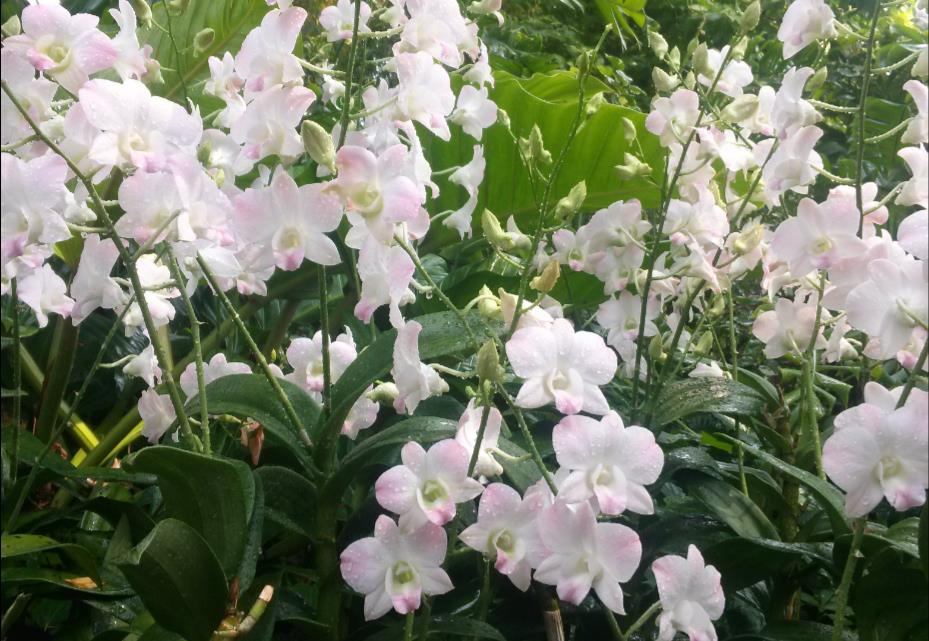
\includegraphics[width=0.5\textwidth]{../gambar/contoh-anggrek.png}
\caption{\textit{Dendrobium Peach}}
\end{figure}

Gambar 2.1 menunjukkan contoh \textit{template} untuk semua gambar yang digunakan di dalam laporan penelitian. Pastikan gambar yang disertakan memiliki resolusi yang mencukupi sehingga gambar dapat dilihat dengan jelas. Gambar adalah hasil gambar (foto) Penulis sendiri. Jika Penulis mengambil gambar dari sumber lain, pastikan untuk menyertakan sitasi (sumber gambar yang diambil). Selalu gunakan \textit{Caption} dan \textit{Cross Reference} dalam memberi nama dan mengacu gambar di dalam \textit{text}.

Gambar 2.2 menunjukkan contoh gambar grafik hasil penelitian. Gambar grafik dapat dibuat berwarna. Gunakan warna yang kontras untuk grafik berwarna yang disertakan. Warna yang kontras akan membuat grafik terlihat jelas saat dicetak berwarna. Ubah warna kontras menjadi garis hitam putih dengan pola titik-titik yang berbeda untuk \textit{hardcopy} hitam-putih. Gambar 2.3 menunjukkan contoh gambar grafik dengan warna hitam-putih. Penomoran gambar dan tabel menggunakan angka Arab, mengikuti urutan bab dan letak gambar/tabel di bab tersebut. Contoh: Gambar 2.2 artinya adalah gambar kedua yang ada di Bab 2, sedangkan Tabel 3.1 artinya adalah tabel pertama yang ada di Bab 3.

\begin{figure}[H]
\centering
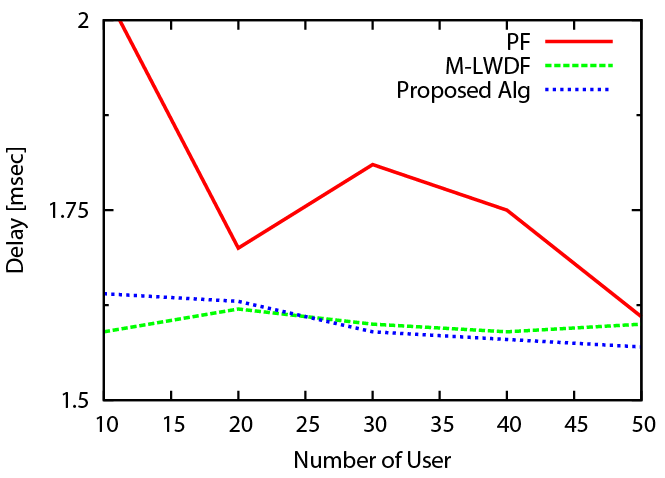
\includegraphics[width=0.55\textwidth]{../gambar/contoh-grafik-warna.png}
\caption{Hasil \textit{delay} warna terhadap penambahan pengguna}
\end{figure}

\begin{figure}[H]
\centering
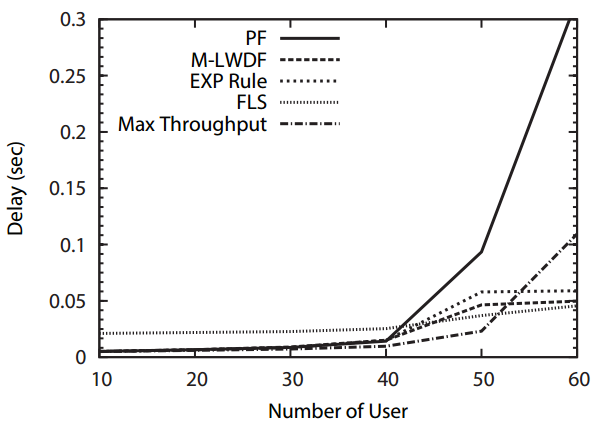
\includegraphics[width=0.55\textwidth]{../gambar/contoh-grafik-monokrom.png}
\caption{Hasil \textit{delay} monokrom terhadap penambahan pengguna}
\end{figure}

\subsection{Sub Tinjauan Teori 2}
\textit{Contoh kalimat bersitasi:} Sumber buku terjemahan ditulis dengan nama penulis aslinya (Gaman \& Sherrington, 1994), artikel berbahasa Indonesia (Radiati, 2000), dan sumber tanpa penulis memakai judul (\textit{Panduan penulisan karya ilmiah}, 2020).

Selalu gunakan perintah masukan persamaan yang disediakan oleh Microsoft Word. Jangan menggunakan potongan (\textit{crop}) persamaan dari literatur lain. Pastikan persamaan yang digunakan tertulis dengan jelas. Contoh \textit{template} persamaan ditunjukkan oleh Persamaan (2.1). Gunakan \textit{Caption} dan \textit{Cross Reference} untuk memudahkan pelacakan dan kompilasi semua persamaan yang digunakan di dalam dokumen. Nomor persamaan harus diletakkan di sisi kanan persamaan. Penggunaan tabel dalam contoh \textit{template} persamaan dimaksudkan untuk memudahkan penulisan \textit{caption} pada sisi kanan persamaan.

\begin{tanpagaris}
\begin{longtable}{@{}p{0.08\linewidth}>{\centering\arraybackslash}p{0.76\linewidth}r@{}}
 & $ds=\sqrt{r^{2}+\left(\dfrac{dr}{d\theta}\right)^{2}}\,d\theta$ & (2.1) \\
\end{longtable}
\end{tanpagaris}

dengan nilai:

\begin{tanpagaris}
\begin{longtable}{@{}p{0.15\linewidth}p{0.05\linewidth}p{0.6\linewidth}@{}}
$ds$ & = & penjelasan 1 \\
$dr$ & = & penjelasan 2 \\
$d\theta$ & = & penjelasan 3 \\
\end{longtable}
\end{tanpagaris}

% Bab 3  Metodologi/Perancangan
\chapter{METODOLOGI/PERANCANGAN}
Bagian ini menjelaskan perancangan sistem yang digunakan, cara mengimplementasikan rancangan, dan cara pengujian sistem (indikator kinerja dan cara mengukurnya). Penjelasan ini bisa terdiri dari beberapa bab yang saling terkait.

\textit{Contoh kalimat bersitasi:} Prosedur pengujian mengacu pada penelitian sebelumnya (AlQahtani \& Alhassany, 2013).

% Bab 4  Jadwal Pelaksanaan
\chapter{JADWAL PELAKSANAAN}
Buatlah jadwal aktivitas berdasarkan tahapan penyelesaian skripsi Anda dalam waktu 6 bulan.

\begin{table}[H]
\caption{Jadwal pelaksanaan penelitian}
\centering
\begin{singlespace}
\renewcommand{\arraystretch}{1.8}
\setlength{\tabcolsep}{9pt}
\begin{tabular}{|c|p{4.8cm}|*{6}{c|}}
\hline
\multirow{2}{*}{\textbf{No}} & \multirow{2}{*}{\textbf{Deskripsi Kegiatan}} & \multicolumn{6}{c|}{\textbf{202x}} \\
\cline{3-8}
 & & 1 & 2 & 3 & 4 & 5 & 6 \\
\hline
1 & Kegiatan 1 & \isi & & & & & \\
\hline
2 & Kegiatan 2 & \isi & \isi & & & & \\
\hline
3 & Kegiatan 3 & & \isi & \isi & & & \\
\hline
4 & Kegiatan 4 & & & \isi & \isi & & \\
\hline
5 & Kegiatan 5 & & & & \isi & & \\
\hline
6 & Kegiatan 6 & & & & & \isi & \isi \\
\hline
\end{tabular}
\end{singlespace}
\end{table}

% Daftar Pustaka (gaya APA edisi ke-7) -- contoh semua jenis sumber
\babtp{DAFTAR PUSTAKA}
Daftar pustaka berisi \textbf{semua} sumber yang dikutip di dalam teks, dan hanya sumber tersebut. Gunakan gaya APA edisi ke-7. Urutkan menurut abjad nama penulis pertama (atau judul bila tanpa penulis), tanpa nomor urut; baris kedua dan seterusnya menjorok ke dalam. Penulis dapat menggunakan bantuan Mendeley atau Zotero untuk menyusun sitasi.

Contoh di bawah mencakup jenis sumber yang umum dipakai: buku, buku terjemahan, bab dalam buku suntingan, artikel jurnal (dengan DOI), prosiding, skripsi atau tesis, laporan lembaga, lembar data (\textit{datasheet}), artikel daring, kode sumber di repositori, dan sumber tanpa penulis. Hapus contoh yang tidak dipakai dan ganti dengan sumber Anda sendiri.

\textbf{Sumber daring dicantumkan tanggal aksesnya.} Untuk laporan daring, artikel daring, dan repositori, akhiri entri dengan \textit{Diakses pada tanggal bulan tahun, dari alamat URL}, karena isinya dapat berubah. Tanggal akses adalah hari saat Anda membuka sumber tersebut. Artikel jurnal yang memiliki DOI cukup ditulis dengan DOI tanpa tanggal akses. Bila tahun terbit tidak diketahui, tulis (t.t.).

Bentuk sitasi di dalam teks untuk jenis sumber di atas:
\begin{itemize}
\item satu penulis: Andrews (2007) atau (Andrews, 2007);
\item dua penulis: (Xu \& Fischione, 2012);
\item tiga penulis atau lebih: (Capozzi et al., 2013);
\item lembaga: (Badan Pusat Statistik, 1997);
\item kutipan langsung dengan halaman: (Ghosh et al., 2010, hlm. 15);
\item tanpa penulis: (\textit{Panduan penulisan karya ilmiah}, 2020).
\end{itemize}

\begin{pustaka}
AlQahtani, S. A., \& Alhassany, M. (2013). Comparing different LTE scheduling schemes. \textit{2013 9th International Wireless Communications and Mobile Computing Conference (IWCMC)}, 264--269.

Andrews, M. (2007). A survey of scheduling theory in wireless data networks. \textit{Wireless Communications, 143}, 1--17.

Badan Pusat Statistik. (1997). \textit{Statistik Indonesia 1996}. Badan Pusat Statistik.

Capozzi, F., Piro, G., Grieco, L. A., Boggia, G., \& Camarda, P. (2013). Downlink packet scheduling in LTE cellular networks: Key design issues and a survey. \textit{IEEE Communications Surveys \& Tutorials, 15}(2), 678--700.

Espressif Systems. (2023). \textit{ESP32-WROOM-32 datasheet} (Versi 3.3) [Lembar data]. \url{https://www.espressif.com/en/support/documents/technical-documents}

Gaman, P. M., \& Sherrington, K. B. (1994). \textit{Ilmu pangan} (M. Gardjito, S. Naruki, Murdiati, \& Sardjono, Penerj.). Gadjah Mada University Press.

Ghosh, A., Zhang, J., Andrews, J. G., \& Muhamed, R. (2010). \textit{Fundamentals of LTE}. Prentice Hall.

Kementerian Komunikasi dan Digital. (2025). \textit{Judul laporan tahunan} [Laporan]. Diakses pada 21 Oktober 2026, dari \url{https://www.komdigi.go.id/contoh-laporan.pdf}

\textit{Panduan penulisan karya ilmiah}. (2020). Penerbit Universitas.

Penulis, A. (2020). Judul bab dalam buku suntingan. Dalam B. Editor \& C. Editor (Ed.), \textit{Judul buku suntingan} (hlm. 10--25). Penerbit.

Penulis, A. B. (2022). \textit{Judul skripsi atau tesis} [Skripsi, Universitas Muhammadiyah Buton]. Repositori Universitas Muhammadiyah Buton. \url{https://repository.example.ac.id/contoh}

Penulis, C. D. (2024). Judul artikel jurnal dengan DOI. \textit{Jurnal Teknologi dan Sistem Komputer, 12}(1), 45--58. \url{https://doi.org/10.xxxx/xxxxx}

Penulis, E. (2026, 5 Maret). Judul artikel berita atau blog. \textit{Nama Situs}. Diakses pada 21 Oktober 2026, dari \url{https://www.contoh.com/artikel}

Penulis, F. (2024). \textit{Nama repositori} [Kode sumber]. GitHub. Diakses pada 21 Oktober 2026, dari \url{https://github.com/pengguna/repositori}

Radiati, L. E. (2000). Penghambatan bakteri enteropatogen oleh ekstrak jahe. \textit{Jurnal Habitat, 12}(2), 81--91.

Xu, Y., \& Fischione, C. (2012). Real-time scheduling in LTE for smart grids. \textit{Proceedings of the 5th International Symposium on Communications, Control and Signal Processing}, 2--4.
\end{pustaka}


\end{document}
